
\chapter{Model}

The implemented model of political competition is the Citizen-Candidate \cite{Osborne1996}, the empirical approach come from \citeA{Elbittar2009}, and Quantal Response Theory (QRE) is used to explain deviations from NE.
In this chapter I present the theoretical model of elections, the Nash Equilibria (NE) in the experimental conditions, and the theory of QRE.
%Few layouts of the empirical methodology are mentioned to clarify NE calculation but the complete empirical methodology is explored at the next chapter.

The Citizen-Candidate model assumes that preferences can be represented in the real line following the Hotelling-Downs's location model. 
It is common to normalize preferences in the $[0,1]$ interval but, given the empirical setup of the model, the $A=[0,100]$ interval is considered.
In the original version of the model, \citeA{Osborne1996} mention that the main results hold even if only a subset of the citizens can be elected whereas the rest just vote. 
The empirical model was implemented in this fashion: the discrete subset $Q={q_1, ..., q_n}, q_i \in A$ represents ideal policies, and each citizen can be referred to by their ideal which is indicated exogenously. 
%The labels "Participant" and "Citizen" are exchangeable. The former will be used when mentioning empirical setups while the later, when discussing the formal model and calculations.

Possible candidates consider the cost of participation $(c)$, the possible benefits of being elected or ego rent $(b)$, and their preferences over the possible final policies implemented. 
In order to model these considerations, equation \ref{Utility} 
represent the preferences of citizens:

\begin{equation}\label{Utility}
	u_i(x,q_i)= -\alpha||x-q_i|| - cs_i + bw_i(s)
\end{equation}

The parameter $\alpha$ indicates the importance of the final policy chosen: proportional to the distance from their ideal point ($q_i$). Thus, citizens prefer policies closer to their locations. The variables $s_i \in \{0,1\}$ and $w_i \in \{0,1\}$ stand for the entry decision ($entry=1$), and the final result ($win=1$), respectively. 
Notice that winning depends on the voting system and the profile of decision made by citizens ($s \in \Pi s_i$), which defines the candidates set.

There are important implications from the decisions' timing and other assumptions that will be now described.

\section{Stages of the Political Process}

Following \citeA{Besley1997} the three stages of the elections are presented in inverse order.
This clarify the subsequent Nash Equilibria calculus as a consequence of backward induction reasoning.

	\subsection{Policy Choice}
	Once having won and holding office, the winner candidate ($q_i^*$) can implement the policy she prefers. 
	At this moment, it is clear that any winner will choose her ideal policy ($x=q_i^*$) maximizing equation \ref{Utility}. Therefore, we can define $x: w \in Q \rightarrow [0,100]$, where $w$ stands for the winner. It will be clear that $x$ is a random variable while $w$ is drawn from a set of candidates.
	
	An important assumption is perfect information: all players know the preferences of others which means that none candidate can cheat about the policy she is going to implement once in office.
	This assumption, and the freedom winner have once in office, contrast with the classical Hotelling-Downs model where candidates are enforced to keep their campaign promises.
	
	\subsection{Voting}
	Given the subset of citizens who have decided to participate in the election ($C \subseteq Q$),
	there is a voting system that designates the winners set ($W: C \rightarrow C$). 
	Plurality Rule (PR) or Run-off (RO) determine function $W$. In both systems, when two or more candidates get the same number of votes, and more than others, they belong to $W$ from were $w$ is randomly sampled.
	These electoral systems are described in section \ref{systems}.
	In both cases, it is assumed that the distribution of voters over $A$ is uniform. Citizens vote sincerely and choose the closer candidate to their own location.  
	The assumption of sincere vote does not allow for coordination between voters. % check for federssen et al 1990
	
	%Then, lets define $P_j(C)$ as the citizen $j$'s probability of being elected.
	%Given that there is a continuum of voters, each citizen represent a single point in $A$, then their own vote choice is negligible\footnote{Remember that there is a continuum of voters from which only a discrete subset of them could be candidates referred to as citizens.}.
	
	\subsection{Entry}
	Each citizen decides simultaneously whether to campaign.
	They do so thinking strategically: considering what other citizens would do evaluating expected payoffs and also thinking strategically. 
	Therefore, the resulting set $C$ is a NE. 
	%Now I continue with the construction of expected utility function.
	
	In the case where no citizen presents a candidacy, everyone receives a payoff of $-D$ which is high enough to deter this case in the equilibrium set. 
	
	Note that the cardinality of $W(C)$ could be more than 1 ($\#((W(C)) \ge 1$). In such a case, the winner is chosen with equal probability due to sincere voting. Then, the citizen $i$'s probability of being elected is defined: $P_i(C)=1/\#((W(C))$ if $q_i \in W(C)$ and $0$ otherwise. 
	Therefore, the winner is a random variable.
	
	In consequence, given the vector of parameters $\theta= (\alpha, c, b, D)$, the expected utility for each citizen can be defined.
	
	\begin{equation}
	U_i( C;\theta )=\Sigma P_j(C)(u_i(x=q_j,q_i;\theta))
	\end{equation}\label{eq:EU}
	
	Because the candidates set is defined from the preceding entry decision ($C=C(S)$), it is convenient to write the expected value as a function of the profiles:
	
	$$
	U_i(s), s \in \Pi_{i \in N} S_i
	$$
	
	From this equation, the existence of a NE can be shown in a standard way using the fixed point theorem.

\section{Electoral Systems}\label{systems}
	\subsection{Plurality Rule}
	In this System, the candidate who get more votes, calculated as in the Hotelling-Downs's location model, is elected. 
	In the case of a tie the winner is chosen randomly as stated before.
	\subsection{Runoff}
	This system take the two candidates with highest votes from a first round, and then a second round of voting is held only with this two options. In the case that one candidate got more that a half of the votes in the first round, she wins without a second round. Winner is chosen randomly if there is a tie in the second round.


\section{Quantal Response Equilibrium}

The Quantal Response Equilibrium (QRE) proposed by \citeA{McKelvey1995} is constructed on the base of a stochastic best response function. The most used implementation is the logistic function over the difference between the expected payoff of the options:

\begin{equation}\label{fn:SBR}
\sigma_{ij}= \displaystyle\frac{e^{(\pi_{j})\lambda}}{e^{(\pi_{j})\lambda}+e^{(\pi_{i\ne j})\lambda} } 
		=\displaystyle\frac{1}{1+e^{(\pi_{i\ne j}-\pi_{j})\lambda }}		
\end{equation}

% lambda interpretation
In this model the parameter $\lambda$ determines the degree of stochasticity of the election. When $\lambda \rightarrow 0$ the election is a fair coin tossing for each option independent of the expected payoffs (minimum level of rationality), and when $\lambda \rightarrow  \infty$ the election is deterministic with the more profitable action being chosen with certainty (complete rationality). 
The expected payoff of action $j$ is represented by $\pi_j$.

An easy way to visualize the effect of $\lambda$ over decisions is to remember the logistic regression: the dependent variable is the probability to choose option $j$, and the independent variable is the difference between expected payoffs of the two options. Intercept is fixed in zero -which imply equal probability when options' expected payoffs are the same-, and slope is precisely $\lambda$, what determines how step is the logistic function. 
For this reason, $\lambda$ is also interpreted as the level of rationality: as it increases, decision will be better in terms of expected payoffs and less uncertain.

% lambda calculus

With equation \ref{fn:SBR} a stochastic best response is defined: 
\begin{equation}
\sigma^*_{ij}(\lambda, \beta, \pi_{j}(\sigma_{-i}))
\end{equation}\label{eq:SBR}
, which is the player $i$'s probability of choose the actions $j$ (i.e. Entry or Not Entry in the Citizen-Candidate model). 
Vector $\beta$ commonly refers to economic parameters that can measure risk aversion or altruism. In the present analysis, I do not consider these possibilities, but because $\beta$ refers to changes in the original payoff matrix, I will use $\beta$ to refer to different games.

With equation \ref{eq:SBR}, a distribution over actions for each player is defined: $$\sigma^*_{i}(\lambda, \beta, \sigma_{-i})$$ 

This stochastic best response have the proprieties of a regular quantal response function stated by \citeA{Goeree2016}:

\begin{itemize}
	\item Interiority: $\sigma_{ij} >0$
	\item Continuity: $\sigma_{ij}$ is continuous and differentiable. 
	\item Responsiveness:  $\partial \sigma_{ij} / \partial \pi_{ij} >0 $
	\item Monotonicity: $\pi_{ij}> \pi_{ik} \Rightarrow \sigma_{ij}>\sigma_{ik}$
\end{itemize}

Notice that stochastic best response is a function of others' mixed strategies ($\sigma_{-i}$). This is the case because, as seen in equation \ref{fn:SBR}, probability depends on $\pi_{j}$ which is a function of others' strategies: $\pi_{j}(\sigma_{-i})$. In the case of the Citizen-Candidate model, $\pi_j$ is the expected payoff of equation \ref{eq:EU}.

Define then the function:
\begin{equation}\label{eq:sigma}
\sigma = (\sigma^*_{1}, ..., \sigma^*_{N})
\end{equation}

Then, quantal response equilibrium ($\sigma^*$) is a fixed point of equation \ref{eq:sigma}, that now is a function only of $\lambda$ and $\beta$. 
Due to the proprieties of the stochastic best response, and using the fixed point theorem, the equilibrium existence is assured. Figure \ref{fig:qrelambda} shows $\sigma^*$ as a function of $\lambda$ for the four games used in the experiment.

% state the problem of finding QRE

Note that a different equilibrium is predicted depending of the value of $\lambda$ and that players tend towards pure strategies as $\lambda$ goes larger. This equilibrium is called logit equilibrium \cite{Goeree2016}. The software Gambit \cite{McKelvey2014} allows to see those equilibria as a function of the rationality parameter $\lambda$. I realized the calculus in \emph{R} \cite{Rpackage} with the package \emph{nleqslv} \cite{Hasselman2011}, and compare the result with gambit's; they are the same. 
%The graphs generated are set in figures \ref{fig:PR_HC_QRE} to \ref{fig:RO_LC_QRE}.



\begin{figure}
\centering
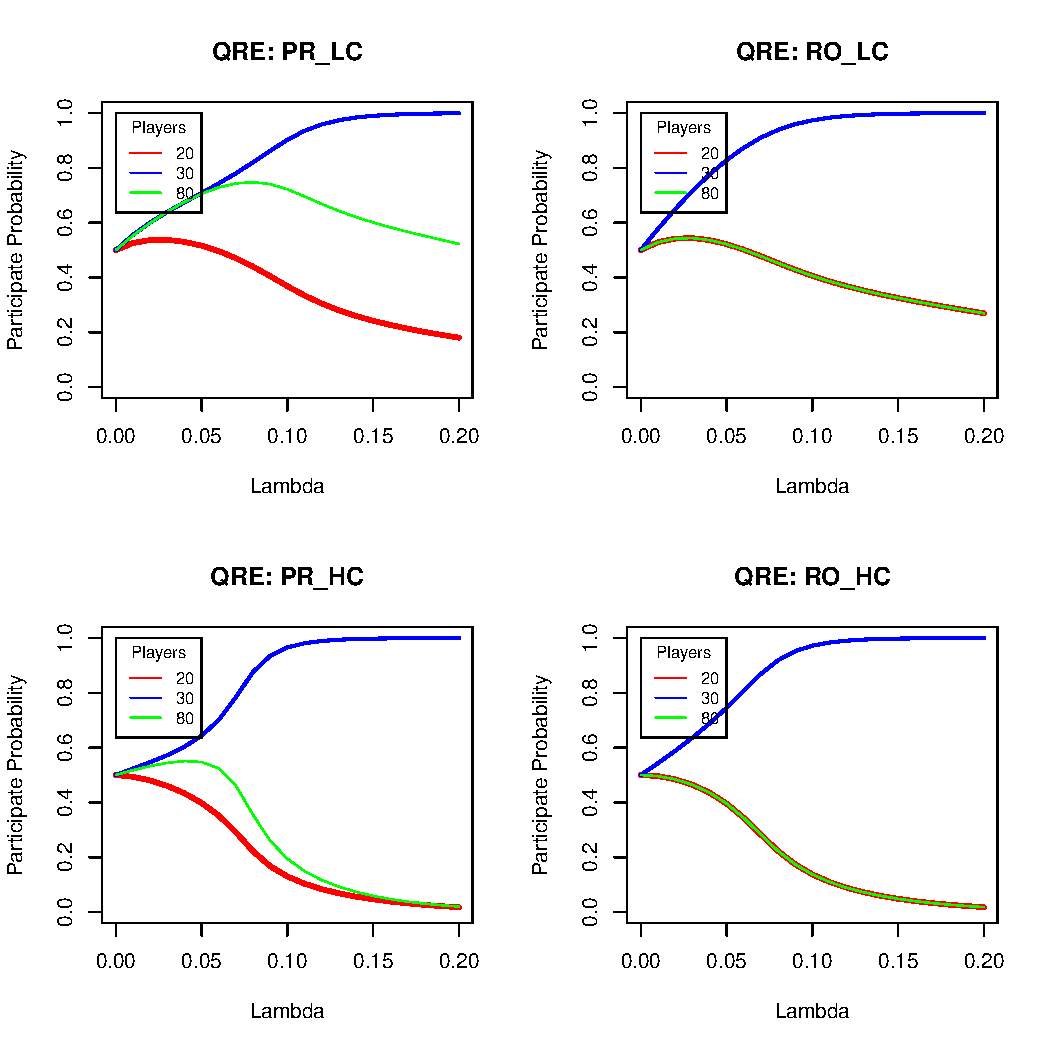
\includegraphics[width=0.7\linewidth]{../../data/QRE_lambda}
\caption[QRE]{Quantal Response Equilibria as function of lambda}
\label{fig:qrelambda}
\end{figure}


The parameter $\lambda$ can be adjusted by maximum likelihood to empirical data as is shown in chapter \ref{chap:res}.

%subsubsectio{Computing Totally Mixed NE}
%It is a well known result that a NE in mixed strategies implies that players are indifferent between the options that have a positive probability to be chosen. The prove just need to consider the other case; if someone were not indifferent, then she would rather prefer one option which contradicts the definition of the NE. 

%In the present game players have two option, which means that if a mixed strategy equilibrium exist every player is indifferent between participate or not. This condition leads to $n$ different equations. Solving this system gives the probability to participate for every player. The solutions could include $\gamma^i \notin [0 ,1]$, which has no sense and those solutions are discarded. 

